% This is LLNCS.DEM the demonstration file of
% the LaTeX macro package from Springer-Verlag
% for Lecture Notes in Computer Science,
% version 2.4 for LaTeX2e as of 16. April 2010
%
\documentclass[a4paper]{llncs}
%

\usepackage{listings}
\usepackage{graphicx}
\usepackage{pgf}
\usepackage{tikz}
\usetikzlibrary{arrows, automata, shapes}


%\usepackage{makeidx}  % allows for indexgeneration
%
\title{Fully Automatic Loop-free Program Synthesis by Bounded Model Checking}
\author{Daniel Kroening \and Matt Lewis}
\institute{University of Oxford}

\newenvironment{keywords}{
       \list{}{\advance\topsep by0.35cm\relax\small
       \leftmargin=0cm
       \labelwidth=0.35cm
       \listparindent=0.35cm
       \itemindent\listparindent
       \rightmargin\leftmargin}\item[\hskip\labelsep
                                     \bfseries Keywords:]}
     {\endlist}

\makeatletter
\pgfdeclareshape{datastore}{
  \inheritsavedanchors[from=rectangle]
  \inheritanchorborder[from=rectangle]
  \inheritanchor[from=rectangle]{center}
  \inheritanchor[from=rectangle]{base}
  \inheritanchor[from=rectangle]{north}
  \inheritanchor[from=rectangle]{north east}
  \inheritanchor[from=rectangle]{east}
  \inheritanchor[from=rectangle]{south east}
  \inheritanchor[from=rectangle]{south}
  \inheritanchor[from=rectangle]{south west}
  \inheritanchor[from=rectangle]{west}
  \inheritanchor[from=rectangle]{north west}
  \backgroundpath{
    %  store lower right in xa/ya and upper right in xb/yb
    \southwest \pgf@xa=\pgf@x \pgf@ya=\pgf@y
    \northeast \pgf@xb=\pgf@x \pgf@yb=\pgf@y
    \pgfpathmoveto{\pgfpoint{\pgf@xa}{\pgf@ya}}
    \pgfpathlineto{\pgfpoint{\pgf@xb}{\pgf@ya}}
    \pgfpathmoveto{\pgfpoint{\pgf@xa}{\pgf@yb}}
    \pgfpathlineto{\pgfpoint{\pgf@xb}{\pgf@yb}}
 }
}
\makeatother



\begin{document}
%
\maketitle
%
\pagestyle{headings}  % switches on printing of running heads

\begin{abstract}
We present a simple-yet-effective method for synthesizing loop-free
programs, using a novel combination of Bounded Model Checking and
explicit-state Model Checking.  The user provides a specification in plain
C, after which the synthesis process is fully automatic.

We demonstrate the effectiveness of our method by synthesizing several subtle
programs acting on machine integers, and a selection of floating-point programs.
\end{abstract}


\begin{keywords}
 Program synthesis, bitvectors, bounded model checking, CBMC,
 floating point.
\end{keywords}

\section{Introduction}

Program synthesis is the mechanized construction of software that provably
satisfies a given specification.  Synthesis tools promise to relieve the
programmer from thinking about \emph{how} the problem is to be solved;
instead, the programmer only provides a compact description of \emph{what}
is to be achieved.  Foundational research in this area has been
exceptionally fruitful, beginning with Alonzo Church's work on the
\emph{Circuit Synthesis Problem} in the sixties~\cite{church-synth}.

In this paper, we present a new method that brings the promise of
automating programming closer to application.  We make pragmatic
restrictions of the general synthesis problem in order to arrive at an
effective solution.  To this end, we focus on the problem of synthesizing
loop-free programs over machine integers and floating-point number from a
specification given as program fragment.

Our work represents a substantial refinement of {\sc brahma}~\cite{brahma},
which is also the closest work to ours.  {\sc Brahma} also focuses on
synthesizing loop-free machine-integer programs.  In~\cite{brahma}, the
authors characterise the program synthesis problem as a second-order
$\exists \forall$ formula, and introduce the CEGIS algorithm for solving
these formulae.  This algorithm reduces the satisfiability of the $\exists
\forall$ formula to the satisfiability of several first-order formulae, each
of which can be decided using an off-the-shelf SMT solver.  {\sc Brahma}
takes as input a specifcation (given as an SMT formula) and a library of
components (one component is more or less a single machine instruction).  It
then finds a permutation of the component library that satisfies the
specification.  This permutation is the final synthesised program.  In the
event that the library does not contain enough components to synthesise a
correct program, the user is told that the library is too small and is
required to add more components until the synthesis succeeds.  Each round of
synthesis amounts to solving an $\exists \forall$ formula that is quadratic
in the size of the component library.

We require the user to supply a program specification written in C, but then
ask nothing more of her.  Our encoding allows us to generate an $\exists
\forall$ formula that is \emph{linear} in the length of the shortest program
satisfying the user's specification, which we then check for satisfiability
using the CEGIS algorithm.  In contrast, the program generated by {\sc
brahma} can be no longer than the size of the library, as the synthesis
outcome is a permutation of the component library.

Another successful approach to program synthesis has been \emph{program
sketching}, in particular the {\sc sketch} tool~\cite{sketch}.  This method
requires the programmer to provide a \emph{program sketch}, written in a
C-like language, together with either a specification (written in the same
language) or a suite of unit tests.  The sketch is a skeleton program which
contains much of the high-level structure of the final program, but with
several ``holes'', which {\sc sketch} fills in to meet the specification,
again using the CEGIS algorithm.

Program synthesis is strongly related to superoptimisation~\cite{superoptimisation},
which is the problem of taking a segment of code, usually written in C, and finding
a minimal program which has the same functionality.  The {\sc aha}~\cite{aha} tool
and the GNU superoptimiser~\cite{gnu-superoptimiser} both perform superoptimisation of
C programs, both by enumerating possible programs and testing them on suitable inputs.
This search can be compiled down to native code using an optimising compiler,
so for short programs the method is extremely fast, however because of the exponential
blowup of the search space it is impractical for synthesising longer programs.
We incorporate this technique by using explicit-state model checking in parallel
with symbolic model checking.

%\paragraph{Outline} We give details of our new algorithm in
%Sec.~\ref{sec:algorithm}. 

\section{The Basic Synthesis Algorithm}
\label{sec:algorithm}

\subsection{The Abstract Algorithm}

Our task is to find a program which satisfies some specifcation.  We can formalize this
notion as follows: fix an input set $I$ and an output set $O$.  Specifications $\sigma$
are then relations and programs $P$ are computable functions:

$$ \sigma \subseteq I \times O $$
$$ P : I \rightarrow O$$

The synthesis problem is then to determine the validity of the following formula, and
to find a witness $P$ if the following second-order formula is valid:

$$\exists P . \forall x \in I . \sigma(x, P(x))$$

Depending on the logic needed to express this formula the synthesis problem may
be decidable, semi-decidable or undecidable.  For many interesting logics, checking
the validity of a second order formula, such as the synthesis formula, is undecidable.
Even for logics in which the problem is decidable, the quantifier alternation means that
we do not have efficient decision procedures to verify our formula, although efficient
methods may exist for solving problems with only one quantifier.  In particular
if we are working in the logic of propositional satisfiability, we have SAT solvers
which are efficient-in-practice at solving queries with a single quantifier.
The corresponding problem with one level of quantifier alternation (2-QBF) is
complete for $NP^{NP}$, and current 2-QBF solvers are much less efficient than SAT solvers.

When the first-order fragment of the logic is efficiently decidable and $P$ can be
expressed as a ground term of the logic, we can use a refinement loop to check the
validity of the synthesis formula as shown in Fig.~\ref{fig:abstract-refinement} and
Fig.~\ref{fig:abstract-refinement-code}.  The algorithm is divided into two
components: {\sc synth} and {\sc verif}.  We track a finite (small) set of inputs
and {\sc synth} synthesizes a candidate program which is correct on just those inputs.
{\sc Verif} then tries to verify the candidate program by searching for an input on
which the candidate program does not satisfy the specification.  If no such input
can be found, the candidate program is correct.  Otherwise, the new input is added
to the set of inputs we must check in {\sc synth}.  If the input set is finite, this
procedure is guaranteed to terminate.

\begin{figure}
 \centering
 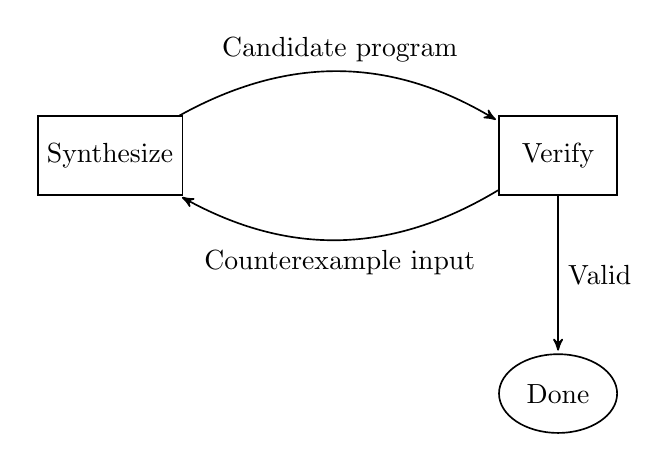
\begin{tikzpicture}[->,>=stealth',shorten >=1pt,auto,
 semithick, initial text=]

  \matrix[nodes={draw, fill=none, scale=1, shape=rectangle, minimum height=1cm, minimum width=1.5cm},
          row sep=2cm, column sep=4cm] {
   \node (synth) {Synthesize};
   &
   \node (verif) {Verify}; \\
   \node[draw=none] {};
   &
   \node[ellipse] (done) {Done}; \\
  };

   \path
    (synth) edge [bend left] node {Candidate program} (verif)
    (verif) edge [bend left] node {Counterexample input} (synth)
    (verif) edge node {Valid} (done);
 \end{tikzpicture}

 \label{fig:abstract-refinement}
 \caption{Abstract synthesis refinement loop}
\end{figure}

\begin{figure}
\centering
\begin{minipage}{0.9\textwidth}
 \begin{lstlisting}[mathescape,language=C]
function synth(inputs) {
  $(i_1, \ldots, i_N)$ = inputs
  query := $\exists P . \sigma(i_1, P(i_1)) \land \ldots \land \sigma(i_N, P(i_N))$
  result := decide(query)
  
  if (result.satisfiable) {
    return result.model
  } else {
    return unsatisfiable
  }
}

function verif(P) {
  query := $\exists x . \lnot \sigma(x, P(x))$
  result := decide(query)
  
  if (result.satisfiable) {
    return result.model
  } else {
    return valid
  }
}

function refinement_loop() {
  inputs := $\emptyset$

  while (true) {
    candidate := synth(inputs)

    if (candidate = unsatisfiable) {
      return unsatisfiable
    }

    res := verif(candidate)

    if (res = valid) {
      return candidate
    } else {
      inputs := inputs $\cup$ res
    }
  }
 \end{lstlisting}
 \end{minipage}

 \label{fig:abstract-refinement-code}
 \caption{Abstract refinement algorithm}
\end{figure}

\subsection{The Concrete Algorithm for Bitvector Programs}

One area in which program synthesis can shine is in producing very small,
intricate programs that manipulate bitvectors.  An example of such a program
is shown in Fig.~\ref{fig:bitvector-program}.  This program takes a machine word
as input and clears every bit except for the least significant bit that was set.
Even though this program is extremely short, it is fairly difficult for a human
to see what it does.  It is even more difficult for a human to come up with such
minimal code -- a natural solution for this problem might be to use a loop which
iterates over all of the bits in the word.  The program is so concise because it
takes advantage of the low level details of the machine, such as the fact that
signed integers are stored in two's complement form.

\begin{figure}
\centering
\begin{minipage}{0.45\linewidth}
 \begin{lstlisting}[language=C]
int isolate_lsb(int x) {
  return x & -x;
}
 \end{lstlisting}
\end{minipage}
\begin{minipage}{0.45\linewidth}
 
Example:

\hrule

\begin{tabular}{llcccccccc}
 x       & = & 1 & 0 & 1 & 1 & 1 & 0 & 1 & 0 \\
 -x      & = & 0 & 1 & 0 & 0 & 0 & 1 & 1 & 0 \\
 x \& -x & = & 0 & 0 & 0 & 0 & 0 & 0 & 1 & 0
\end{tabular}
\end{minipage}

 \label{fig:bitvector-program}
 \caption{A tricky bitvector program}
\end{figure}

To synthesize tricky bitvector programs like this, it is natural for us to work
in the logic of quantifer free propositional formulae and to use a SAT solver as
the decision procedure.  However, we propose a slightly different tack, which is
to use a decidable fragment of C as our underlying logic.  The fragment we use
has the following restrictions:

\begin{itemize}
 \item All loops and recursive function calls must terminate after a constant number
 of iterations.  This constant must be statically inferrable.
 \item Arrays must all be statically allocated with a constant size.
\end{itemize}

Other than this any C constructs can be used, which still leaves a very expressive
language with the nice property that safety is decidable using a single query to a
bounded model checker.  We will refer to this fragment as C-.  To instantiate the
abstract synthesis algorithm in C- we must express $I, O, \sigma$ and $P$ in C-,
then ensure that we can express the validity of the synthesis formula as a safety
property of the resulting C- program.

Our encoding is the following:

\begin{itemize}
 \item $I$ is the type \verb|int[N]|.
 \item $O$ is the type \verb|int[M]|.
 \item $\sigma$ is a function with signature
 \verb|int check(int in[N], int out[M])|. This function is the only component supplied
 by the user.
 \item $P$ is written in a simple RISC language $\mathcal{L}$.  Programs in $\mathcal{L}$
 have the type \verb|prog_t|.
 \item We supply an interpreter for $\mathcal{L}$ which is written in C-.  The signature
 of this interpreter is \\
 \verb|void exec(prog_t p, int in[N], int out[M])|.
\end{itemize}

\begin{figure}
\centering
\begin{minipage}{0.65\textwidth}
\setlength{\tabcolsep}{16pt}
Integer arithmetic instructions:

\begin{tabular}{lll}
 \verb|add a b| & \verb|sub a b| & \verb|mul a b| \\
 \verb|div a b| & \verb|neg a|
\end{tabular}
\bigskip

Bitwise logical and shift instructions:

\begin{tabular}{lll}
 \verb|and  a b| & \verb|or   a b| & \verb|xor  a b| \\
 \verb|ashr a b| & \verb|lshr a b| & \verb|not  a|
\end{tabular}
\bigskip

Unsigned and signed comparison instructions:

\begin{tabular}{lll}
 \verb|le  a b| & \verb|lt  a b| & \verb|sle  a b| \\
 \verb|slt a b|
\end{tabular}
\end{minipage}

 \label{fig:l-language}
 \caption{The language $\mathcal{L}$}
\end{figure}

We must now express the {\sc synth} and {\sc verif} formulae as safety properties
of C- programs, which is shown in Fig.~\ref{fig:c-synthverif}.

\begin{figure}
\centering
\begin{minipage}{0.45\textwidth}
\begin{lstlisting}[language=C++]
void synth() {
  prog_t p = nondet();
  int in[N], out[M];
  
  in = test1;
  exec(p, in, out);
  assume(check(in, out));
  
  ...
  
  in = testN;
  exec(p, in, out);
  assume(check(in, out));
  
  assert(false);
}
\end{lstlisting}
\end{minipage}
\begin{minipage}{0.45\textwidth}
\begin{lstlisting}[language=C]
void verif(prog_t p) {
  int in[N] = nondet();
  int out[M];

  exec(p, in, out);
  assert(check(in, out));
}
\end{lstlisting}
\end{minipage}

 \label{fig:c-synthverif}
 \caption{The {\sc synth} and {\sc verif} formulae expressed as a C- program}
\end{figure}

\begin{figure}
\begin{center}
\begin{tikzpicture}[
  scale=0.8,
  font=\sffamily,
  every matrix/.style={ampersand replacement=\&,column sep=.5cm,row sep=.75cm},
  source/.style={draw,thick,rounded corners,fill=yellow!20,inner sep=.3cm},
  process/.style={draw,thick,circle,fill=blue!20},
  sink/.style={source,fill=green!20},
  datastore/.style={draw,very thick,shape=datastore,inner sep=.3cm},
  dots/.style={gray,scale=2},
  to/.style={->,>=stealth',shorten >=1pt,semithick,font=\sffamily\footnotesize},
  every node/.style={align=center, scale=0.8}]

  % Position the nodes using a matrix layout
  \matrix{
    \& \node[source] (driver) {driver}; \& \node[source] (user) {user}; \& \\
    \& \node[datastore] (tests) {\texttt{tests.c}}; \& \node[datastore] (spec) {\texttt{spec.c}}; \& \node[datastore] (interpreter) {\texttt{interpreter.c}}; \\
    \node[datastore] (cbmc-synth) {\texttt{cbmc/synth.c}}; \& \node[process] (cbmc) {\sc cbmc}; \& \node[process] (gcc) {\sc gcc}; \& \node[datastore] (explicit-synth) {\texttt{explicit/synth.c}}; \\
    \& \& \node[process] (aout) {\texttt{a.out}}; \& \\
    \& \node[sink] (cbmc-out) {candidate program}; \& \node[sink] (explicit-out) {candidate program}; \& \\
  };

  \draw[to] (driver) -- (tests);
  \draw[to] (user) -- (spec);

  \draw[to] (tests) -- (cbmc);
  \draw[to] (spec) -- (cbmc);
  \draw[to] (interpreter) -- (cbmc);

  \draw[to] (tests) -- (gcc);
  \draw[to] (spec) -- (gcc);
  \draw[to] (interpreter) -- (gcc);
  
  \draw[to] (cbmc-synth) -- (cbmc);
  \draw[to] (explicit-synth) -- (gcc);
  
  \draw[to] (gcc) -- (aout);
  
  \draw[to] (cbmc) -- (cbmc-out);
  \draw[to] (aout) -- (explicit-out);
\end{tikzpicture}
\end{center}

\label{fig:synth-dfd}
\caption{Schematic diagram of {\sc synth}}
\end{figure}


\begin{figure}
\begin{center}
\begin{tikzpicture}[
  scale=0.8,
  font=\sffamily,
  every matrix/.style={ampersand replacement=\&,column sep=.5cm,row sep=.75cm},
  source/.style={draw,thick,rounded corners,fill=yellow!20,inner sep=.3cm},
  process/.style={draw,thick,circle,fill=blue!20},
  sink/.style={source,fill=green!20},
  datastore/.style={draw,very thick,shape=datastore,inner sep=.3cm},
  dots/.style={gray,scale=2},
  to/.style={->,>=stealth',shorten >=1pt,semithick,font=\sffamily\footnotesize},
  every node/.style={align=center, scale=0.8}]

  % Position the nodes using a matrix layout
  \matrix{
    \& \node[source] (driver) {driver}; \& \node[source] (user) {user}; \& \\
    \& \node[datastore] (prog) {\texttt{prog.c}}; \& \node[datastore] (spec) {\texttt{spec.c}}; \& \node[datastore] (interpreter) {\texttt{interpreter.c}}; \\
    \node[datastore] (cbmc-verif) {\texttt{cbmc/verif.c}}; \& \node[process] (cbmc) {\sc cbmc}; \& \node[process] (gcc) {\sc gcc}; \& \node[datastore] (explicit-verif) {\texttt{explicit/verif.c}}; \\
    \& \& \node[process] (aout) {\texttt{a.out}}; \& \\
    \& \node[sink] (cbmc-out) {test vector}; \& \node[sink] (explicit-out) {test vector}; \& \\
  };

  \draw[to] (driver) -- (prog);
  \draw[to] (user) -- (spec);

  \draw[to] (prog) -- (cbmc);
  \draw[to] (spec) -- (cbmc);
  \draw[to] (interpreter) -- (cbmc);

  \draw[to] (tests) -- (gcc);
  \draw[to] (spec) -- (gcc);
  \draw[to] (interpreter) -- (gcc);
  
  \draw[to] (cbmc-verif) -- (cbmc);
  \draw[to] (explicit-verif) -- (gcc);
  
  \draw[to] (gcc) -- (aout);
  
  \draw[to] (cbmc) -- (cbmc-out);
  \draw[to] (aout) -- (explicit-out);
\end{tikzpicture}
\end{center}

\label{fig:verif-dfd}
\caption{Schematic diagram of {\sc verif}}
\end{figure}


\section{C-}
We use a fragment of C as our underlying logic.  We will refer to this fragment
as C-.  The characteristic property of C- is that safety can be decided for
C- programs by using a bounded model checker.  A C- program is just a C program
with the following syntactic restrictions:

\begin{itemize}
 \item All loops in the program must have a constant bound.
 \item All recursion in the program must be limited to a constant depth.
 \item All arrays must be statically allocated (i.e. not using \texttt{malloc}),
 and be of constant size.
\end{itemize}

Additionally, C- programs may use:

\begin{itemize}
 \item Nondeterministic values.
 \item Assumptions.
 \item Arbitrary width types.
\end{itemize}

So for example the programs in Fig.~\ref{fig:c-} are valid
C- programs, but the program in Fig.~\ref{fig:not-c-} is not, since it uses
a non-constant loop bound.

\begin{figure}
\begin{minipage}[scale=0.8]{0.45\linewidth}
 \begin{lstlisting}[language=c]
int count_bits(int x) {
  int i, ret;
  
  ret = 0;
  
  for (i = 0; i < 32; i++) {
    if (x & (1 << i))
      ret++;
  }
  
  return ret;
}
 \end{lstlisting}
\end{minipage}
\begin{minipage}{0.54\linewidth}
 \begin{lstlisting}[language=C]
int common_factor(int A[10]) {
  int factor = nondet();
  int i;

  for (i = 0; i < 10; i++) {
    assume((A[i] % factor) == 0);
  }

  assume(factor > 1);
  return factor;
}

 \end{lstlisting}
\end{minipage}

 \label{fig:c-}
 \caption{Two C- programs.}
\end{figure}

\begin{figure}
 \begin{lstlisting}[language=C]
int fib(int n) {
  int a, b, c;
  
  a = b = 1;
  
  while (n--) {
    c = a+b;
    a = b;
    b = c;
  }
  
  return a;
}
 \end{lstlisting}

 \label{fig:not-c-}
 \caption{A C program to compute Fibonacci numbers.}
\end{figure}

Since each loop is bounded by a constant, and each recursive function call is
limited to a cosntant depth, a C- program necessarily terminates and in
fact does so in $O(1)$ time.  If we call the largest loop bound $k$, then
a bounded model checker with an unrolling bound of $k$ will be a complete
decision procedure for the safety of the program.  For a C- program of
size $l$ and with largest loop bound $k$, a bounded model checker will
create a SAT problem of size $O(lk) = O(l)$.  Conversely, a SAT problem
of size $s$ can be converted trivially into a loop free C- program
of size $O(s)$.  The safety problem for C- is therefore NP-complete,
which means it can be decided fairly efficiently for many practical
instances.

\subsection{Why use C- instead of SAT?}
To misquote David Wheeler: ``all problems in computer science can be solved by
another level of abstraction.''~\cite{beautiful-code}.  C- serves as
an abstraction of SAT.  We can think of SAT as an assembly language and
{\sc cbmc} as a compiler for C- to this assembly language.  The benefits
of using C- as our logic rather than SAT are very similar to the benefits of
writing code in a high level language rather than assembly language.
Some of the more significant advantages are:

\begin{itemize}
 \item The code is more readable and easier to debug.
 \item The code is much more concise.
 \item We can take advantage of new optimisations, different model
 checkers and different backends (SAT, SMT, ACDCL, etc.) for free.
\end{itemize}

To illustrate some of these points, we were able to implement a first
version of {\sc kalashnikov} in around 150 lines of code, which took
around two hours to write.  The resulting code was easy to modify,
optimise and debug.  The current version, which includes floating point
support, several optimisations and two model checking algorithms,
is still less than 1200 lines of code (600 lines of C- and 600 lines
of Python).

Another benefit of using C- as our logic is that it would be easy to
automatically extract specifications from C programs, which would be
useful in the context of superoptimisation.  This is because C- is
a relatively large fragment of C, so we anticipate that many interesting
sections of real code will already be C-.

\section{Optimizations}

By far the dominant factor in the total runtime of the synthesis algorithm is
the runtime of {\sc synth}.  It is not entirely surprising that this runtime
is strongly related to the size of the SAT problem generated by CBMC.  The size
of the SAT problem is influenced by the number of bits needed to encode $P$,
and by the number of bits needed to encode a run of the $\mathcal{L}$-interpreter.
The connection to Kolmogorov complexity is fairly obvious.

The most successful optimizations we found were related to making fragments of
$\mathcal{L}$ and searching progressively larger fragments until a program
could be found.

\subsection{Limited Program Length}
The simplest restriction on programs is to only consider programs of a certain length.
We start by considering programs consisting of one instruction and progressively
increase this number.

\subsection{Word Width}
It is often the case that a program which satisfies the specification
will continue to satisfy it regardless of the word width of the machine it is
impemented on.  For example the program in Fig.~\ref{fig:bitvector-program}
isolates the least significant bit of an 8-bit word, but it will also
isolate the least significant bit of a 32-bit or indeed any sized word.

Because of this, we can often find a program that is correct for a large
word size by synthesizing a program for a machine with a smaller word size.
This reduces the size of all the constants in the program, the search space
of possible test inputs and also the size of all the state variables internal
to the $\mathcal{L}$-interpreter.

The only wrinkle here is that sometimes a program we synthesize will contain
constants.  If we have synthesized a program for a machine with $k$-bit words,
the constants in the program will be $k$ bits wide.  To generalize the program
to a $n$-bit machine (with $n > k$), we need some way of deriving $n$-bit
wide numbers from $k$-bit ones.  We have several strategies for this and
just try each in turn.  In the following, a subscript $n$ on a value means that
the value is an $n$-bit word.  The dot operator $a_l \cdot b_m$ denotes
concatenation, resulting in an $(l+m)$-bit wide word.  A superscript on a value
means duplication, so $a_l^m$ means concatenating together $m$ copies of the $l$-bit
word $a$, resulting in an $(lm)$-bit wide word.

To generalize a number $x$ we use the following rules:

\begin{itemize}
 \item If $x = k_k$, generalize to $n_n$.
 \item If $x = k-1_k$, generalize to $n-1_n$.
 \item If $x = k+1_k$, generalize to $n+1_n$.
 \item Generalize $x_k$ to $x_n$.
 \item Generalize $x_k$ to $x_k \cdot 0_{n-k}$.
 \item Generalize $x_k$ to $x_k^{n / k}$.
\end{itemize}


\subsection{Separate Constants}
$\mathcal{L}$ is a SSA, three address instruction set.  Destination registers
are implicit and a fresh register exists for each instruction to write its
output to.  A natural way to encode $\mathcal{L}$ instructions is to have an
opcode and two operands.  The opcode selects which instruction type is being
executed and the operands specify which registers should be operated on.
We might allow the operands to be either a register (i.e. a program argument
or the result of a previous instruction), or an immediate constant.

Each opcode requires $\log_2 I$ bits to encode, where $I$ is the number
of instruction types in $\mathcal{L}$.  Each operand can be encoded using
$\log_2 w$ bits, where $w$ is the $\mathcal{L}$-machine word, plus one
bit to specify whether the operand is a register name or an immediate constant.
One instruction can therefore be encoded using $\log_2 I + 2w + 2$ bits.
For an $n$ instruction program, we need $$n \log_2 I + 2nw + 2n$$ bits to encode
the entire program.

If we instead limit the number of constants that can appear in the program,
our operands can be encoded using fewer bits.  For an $n$ instruction program
using $k$ constants and taking $a$ arguments as inputs, each operand can refer
to a program argument, the result of a previous instruction or a constant.
This can be encoded using $\log_2 (k+a+n-1)$ bits, which means each instruction
can be encoded in $\log_2 I + \log_2 (k + a + n - 1)$ and the full program
needs $$n \log_2 I + n \log_2 (k + a + n - 1) + kw$$ bits to encode.

To give an example, $\mathcal{L}$ has 15 instruction types, so each opcode is 4 bits.
For a 10 instruction program over 1 argument, using 2 constants on a 32-bit word
machine the first encoding requires $10 * (4 + 32 + 1 + 32 + 1) = 700$ bits.
Using the second encoding, each operand can be represented using
$\log_2 (2 + 1 + 10 - 1) = 4$ bits, and the entire program requires 184 bits.
This is a substantial reduction in size and when the required program requires
few constants this can lead to a very significat speed up.

As with program length we can progressively increase the number of constants in
our program.  We start by trying to synthesize a program with no constants, then
if that fails we try to synthesize using one constant and so on.

\subsection{Explicit Search}
When we are working on an $\mathcal{L}$-machine with a small word size and
a compact program encoding, our state space is very small.
We can quickly check the validity of the {\sc synth} and {\sc verif} formulae
by simply enumerating all of the inputs and programs, then explicitly
executing each program on each input.

Since everything in our system is written in C, we can add a simple loop
to enumerate all programs and inputs, then compile the code using {\sc gcc}.
The resulting binary will explicitly search for programs satisfying the {\sc synth}
formula, or for counterexamples satisfying the {\sc verif} formula.
For small state spaces, these explicit search binaries are often faster
than symbolically evaluating the {\sc synth} and {\sc verif} formulae with
{\sc CBMC}.

\subsection{Remove nops}
Many instructions in $\mathcal{L}$ are nops that do not doing anything.
For example the instruction \verb|add x 0| does nothing.  Such instructions
can be removed from any program they appear in to leave a semantically
equivalent, but shorter, program.  We can therefore be sure that nops
will never appear in any minimal program.  By adding constraints saying that
each instruction is not a nop, we can help the underlying SAT solver's
search, which reduces the runtime of the overall procedure.

\subsection{Symmetry Reduction}
There are many instructions that are equivalent to each other.  For example,
\verb|add x y| is equivalent to \verb|add y x| -- any program containing
one instruction could have it replaced by the other instruction and
keep the same semantics.  We choose a single canonical instruction to
represent all instructions in a particular equivalence class, then add
constraints saying that no non-canonical instructions appear in the program.

Our rules for excluding non-canonical instructions are:

\begin{itemize}
 \item For commutative operations, the first operand is smaller than the second.
 \item For unary operations, the second (unused) operand is always 0.
 \item No instruction may have two constant operands.
 \item All program constants are distinct.
\end{itemize}

As with the nop constraints, these additional constraints do increase the
size of the resulting SAT instance, but this still ends up as a win in
terms of runtime.

\subsubsection{Implementing $\mathcal{L}$ With A Stack Machine}
Three-address code tends to be less compact than code written for a stack
machine.  It therefore would seem reasonable to use a stack machine to
execute $\mathcal{L}$ programs, since we would expect to see smaller programs
(in terms of bits used in the encoding), leading to smaller SAT instances
and faster runtimes overall.

Unfortunately we saw quite the opposite effect -- runtimes when implementing the
$\mathcal{L}$-interpreter as a stack machine were much higher than the three-address
code implementation.  We believe the reason for this
effect is that the internal state of a stack based interpreter is much more complex
to analyse than an interpreter for three-address code.  This is because a
three-address code interpreter can be implemented using a single array whose cells are
each written to exactly once (each cell corresponds to a register in the program).
By contrast a stack machine interpreter has a stack as its central data structure.
It is natural to implement this as an array, but the array's contents are accessed
in an unpredictable, non-uniform manner as the stack pointer increases and decreases
over the lifetime of the program.  This leads to a \emph{larger} SAT
instance and drastically slows down the operation of the solver.

\begin{figure}
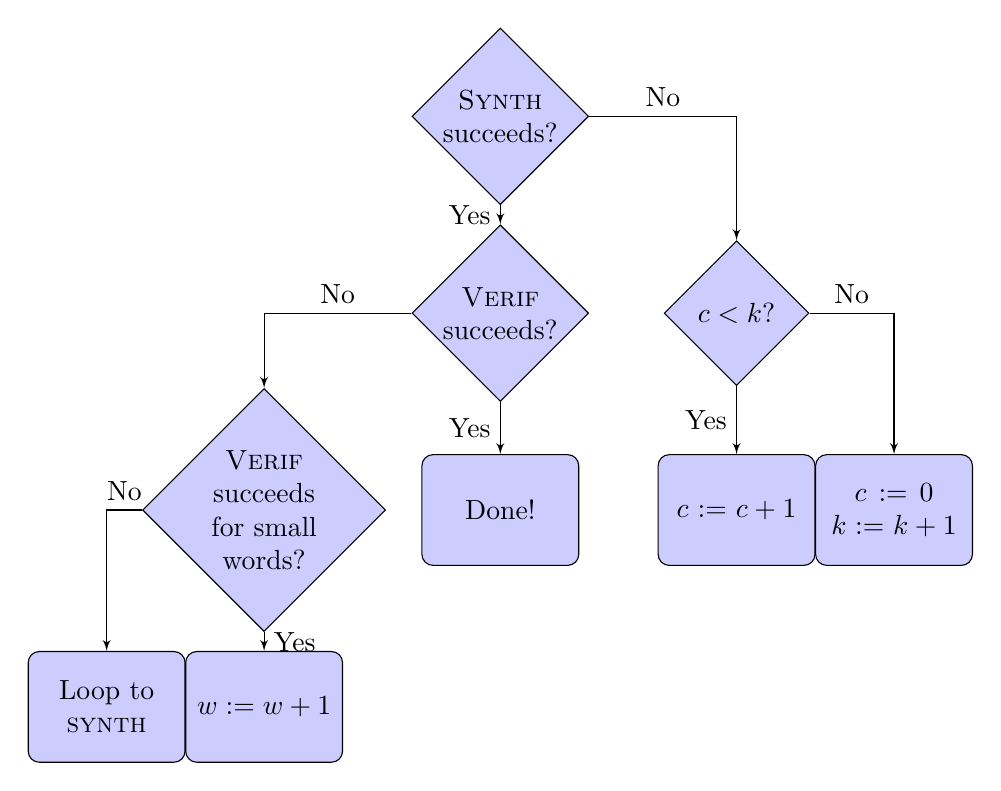
\begin{tikzpicture}{node distance=2cm, auto}
\tikzstyle{decision} = [diamond, draw, fill=blue!20, 
    text width=4.5em, text badly centered, node distance=3cm, inner sep=0pt]
\tikzstyle{block} = [rectangle, draw, fill=blue!20, 
    text width=5em, text centered, rounded corners, minimum height=4em]
\tikzstyle{line} = [draw, -latex']
\tikzstyle{cloud} = [draw, ellipse,fill=red!20, node distance=3cm,
    minimum height=2em]

 \node [decision] (synthsucc) {{\sc Synth} succeeds?};

 \node [decision, below of=synthsucc, node distance=2.5cm] (verif) {{\sc Verif} succeeds?};
 \node [decision, right of=verif] (ck) {$c < k$?};

 \node [block, below of=verif, node distance=2.5cm]   (done) {Done!};
 \node [decision, left of=done] (verifw) {{\sc Verif} succeeds for small words?};

 \node [block, below of=ck, node distance=2.5cm] (incc) {$c := c+1$};
 \node [block, right of=incc, node distance=2cm] (inck) {$c := 0$\\ $k := k+1$};

 \node [block, below of=verifw, node distance=2.5cm] (incw) {$w := w+1$};
 \node [block, left of=incw, node distance=2cm] (iterate) {Loop to {\sc synth}};

 \path [line] (synthsucc) -- node [left] {Yes} (verif);
 \path [line] (synthsucc) -| node [above, near start] {No} (ck);

 \path [line] (verif) -- node [left] {Yes} (done);
 \path [line] (verif) -| node [above, near start] {No} (verifw);

 \path [line] (ck) -- node [left] {Yes} (incc);
 \path [line] (ck) -| node  [above, near start]  {No}(inck);

 \path [line] (verifw) -- node [right] {Yes} (incw);
 \path [line] (verifw) -| node [above, near start] {No} (iterate);
\end{tikzpicture}

\label{fig:paramsflow}
 \caption{Decision tree for increasing parameters of $\mathcal{L}$.}
\end{figure}

\section{Floating Point}

\begin{figure}
 \begin{lstlisting}[language=c]
s  = a + b;
b2 = s - a;
a2 = s - b2;
db = b - b2;
da = a - a2;
t  = da + db;
 \end{lstlisting}

\begin{lstlisting}[language=c]
s = a + b;
z = s - a;
t = b - z;
\end{lstlisting}

 
 \label{fig:2sum}
 \caption{2Sum}
\end{figure}


\section{Experimental Results}

We performed our experiments on a 4-core, 3.07GHz Xeon X5667 with 50GB of RAM.

\begin{figure}
\begin{center}
\begin{tabular}{l|l|l|l|l}
Problem & {\sc Brahma} & {\sc Kalashnikov} & {\sc Kalashnikov} & {\sc Kalashnikov} \\
        &               &                    & (no width)         & (CBMC only) \\
\hline
p1 & 3.20s &{\bf 1.83s} &23.54s &8.07s \\
p2 & 3.60s &{\bf 1.49s} &1271.12s &8.19s \\
p3 & {\bf 1.40s} &1.60s &4.09s &5.90s \\
p4 & 3.30s &{\bf 1.86s} &79.72s &8.15s \\
p5 & 2.20s &{\bf 1.98s} &12.16s &8.10s \\
p6 & 2.40s &{\bf 1.51s} &104.19s &8.17s \\
p7 & {\bf 1.00s} &4.04s &- &14.49s \\
p8 & {\bf 1.40s} &4.31s &- &14.20s \\
p9 & {\bf 5.80s} &35.09s &505.10s &13.45s \\
p10 & 76.10s &{\bf 9.80s} &- &19.14s \\
p11 & 57.10s &{\bf 9.40s} &{\bf 9.40s} &32.98s \\
p12 & 67.80s &{\bf 21.43s} &{\bf 21.43s} &38.23s \\
p13 & 59.60s &27.74s &27.74s &{\bf 13.16s} \\
p14 & 118.90s &54.71s &54.71s &{\bf 52.69s} \\
p15 & 62.30s &{\bf 43.49s} &{\bf 43.49s} &44.31s \\
p16 & 78.10s &{\bf 27.41s} &{\bf 27.41s} &45.84s \\
p17 & 45.90s &{\bf 27.73s} &{\bf 27.73s} &46.63s \\
p18 & 34.70s &{\bf 5.55s} &{\bf 5.55s} &15.63s \\
p19 & {\bf 108.40s} &- &- &- \\
p20 & {\bf 28.30s} &- &- &- \\
p21 & {\bf 279.00s} &- &- &- \\
p22 & {\bf 1668.00s} &- &- &- \\
p23 & {\bf 224.90s} &- &- &- \\
p24 & {\bf 2778.70s} &- &- &- \\
\end{tabular}

\end{center}

\label{fig:results-table}
\caption{Times for synthesis of machine integer benchmarks from {\sc brahma} paper}
\end{figure}


\begin{figure}
 \includegraphics[width=\linewidth]{figures/brahma_kalashnikov.pdf}
 \label{fig:brahma-kalashnikov}
 \caption{Brahma runtimes vs. Kalashnikov}
\end{figure}


\section{Conclusion}

\bibliography{synth}{}
\bibliographystyle{splncs}

\end{document}
